\documentclass{scrartcl}
\usepackage[sexy]{evan}
\usepackage{graphicx} % Required for inserting images

\title{CS230 Notes (Quiz-2)}
\author{Soham Joshi}
\date{March 2023}

\begin{document}

\maketitle

\section{Summary}

\begin{figure}[h]
\centering
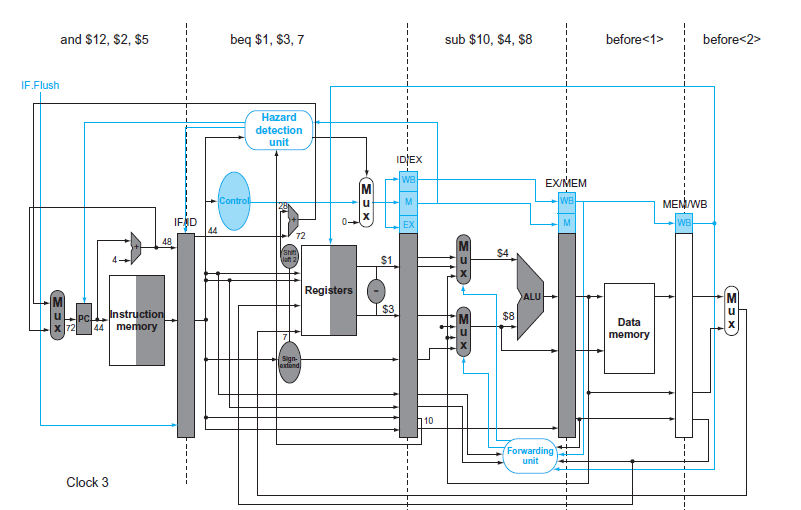
\includegraphics[scale=0.8]{Images/branch_dec_to_ID.png}
\caption{Shifting branch decision to ID stage}
\end{figure}

\begin{figure}[h]
\centering
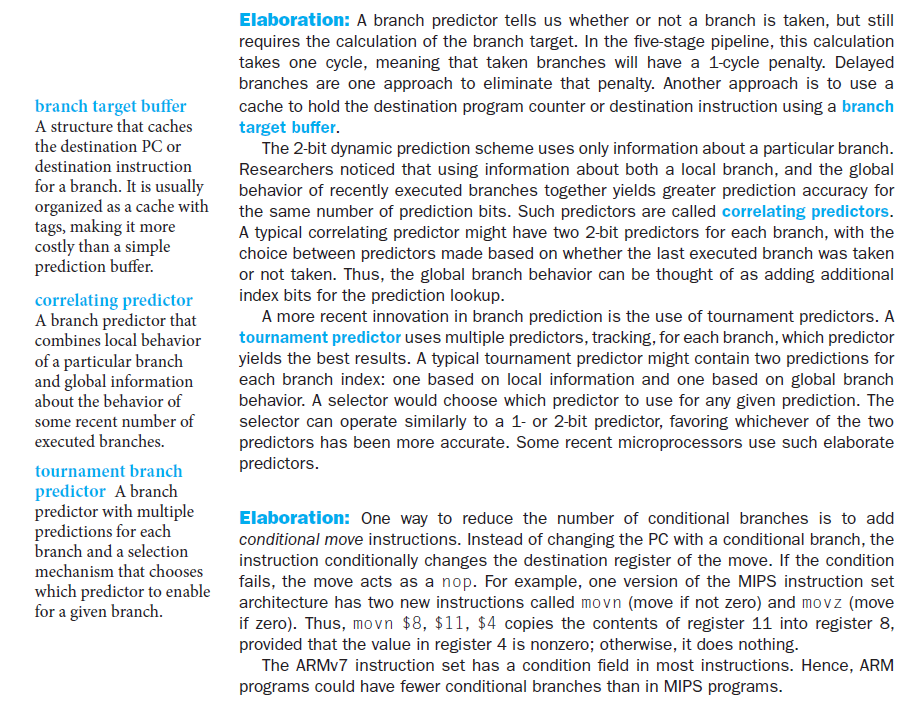
\includegraphics[scale=0.6]{Images/BTB_predictors.png}
\caption{Branch predictors (types)}
\end{figure}

\begin{figure}[h]
\centering
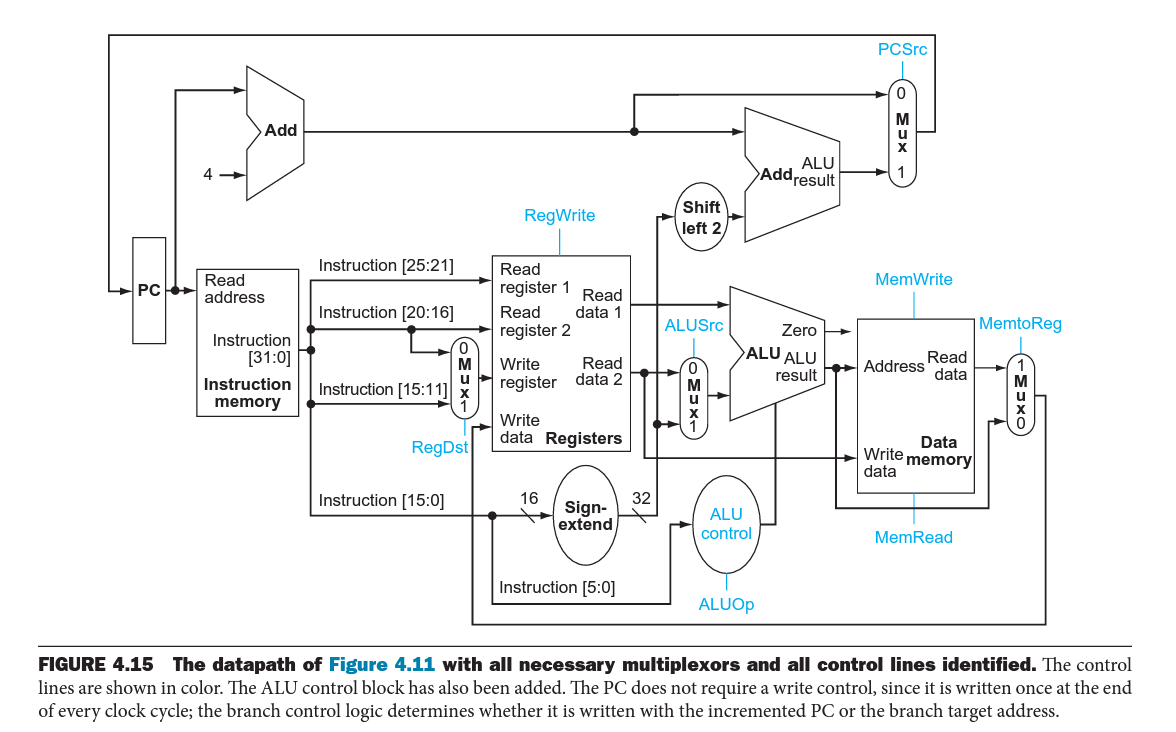
\includegraphics[scale=0.5]{Images/complete_path.png}
\caption{Single cycle CPU}
\end{figure}

\begin{figure}[h]
\centering
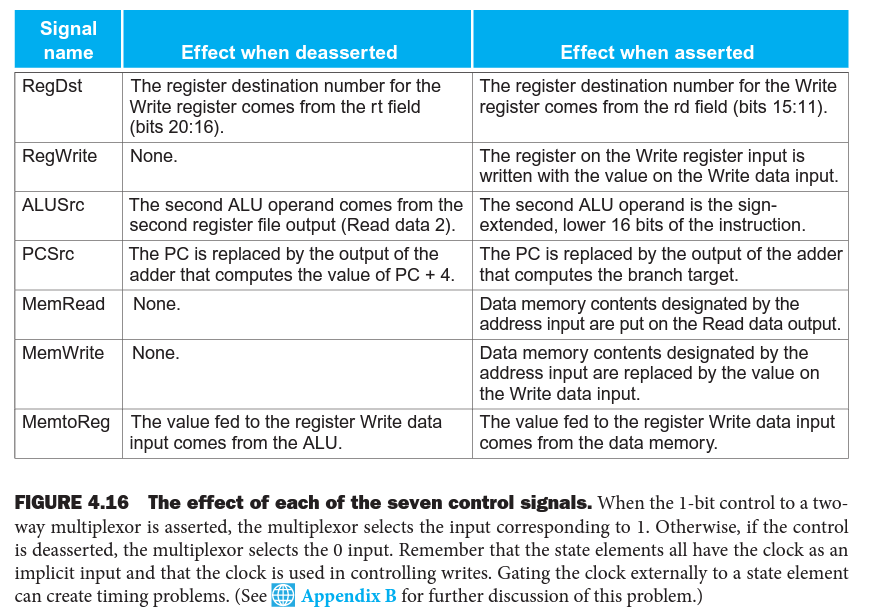
\includegraphics[scale=0.5]{Images/control_signals.png}
\caption{Control signals for pipeline}
\end{figure}

\begin{figure}[h]
\centering
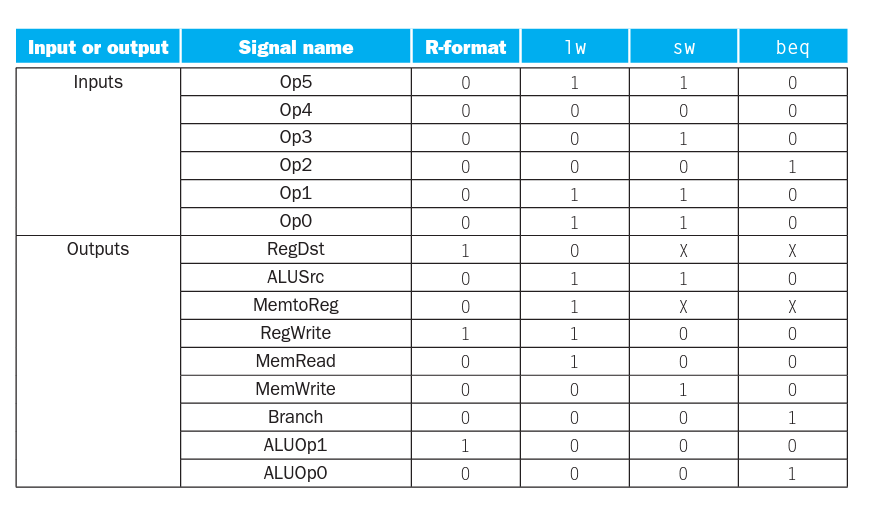
\includegraphics[scale=0.5]{Images/control_summary.png}
\caption{Control signals for pipeline (values)}
\end{figure}

\begin{figure}[h]
\centering
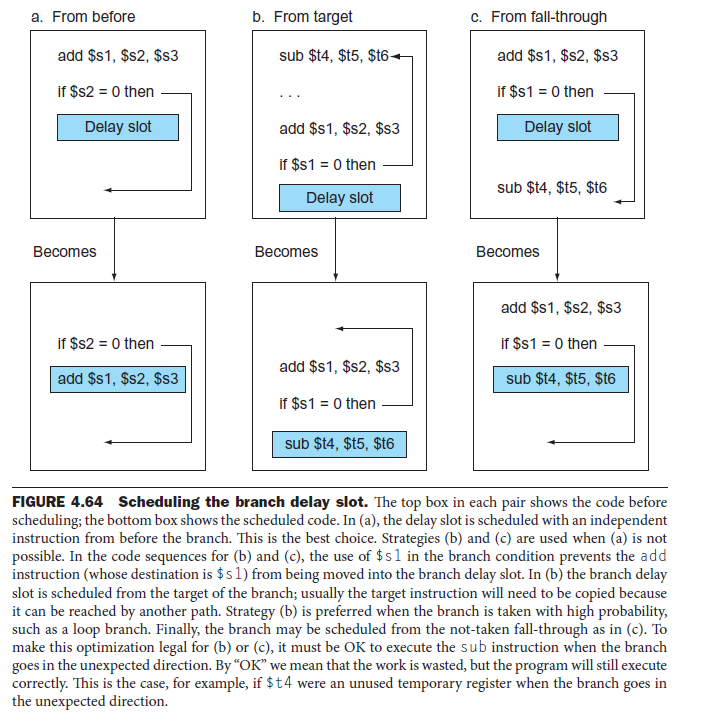
\includegraphics[scale=0.7]{Images/delay_slot.png}
\caption{Delay slots as a method for branch control hazard mitigation}
\end{figure}

\begin{figure}[h]
\centering
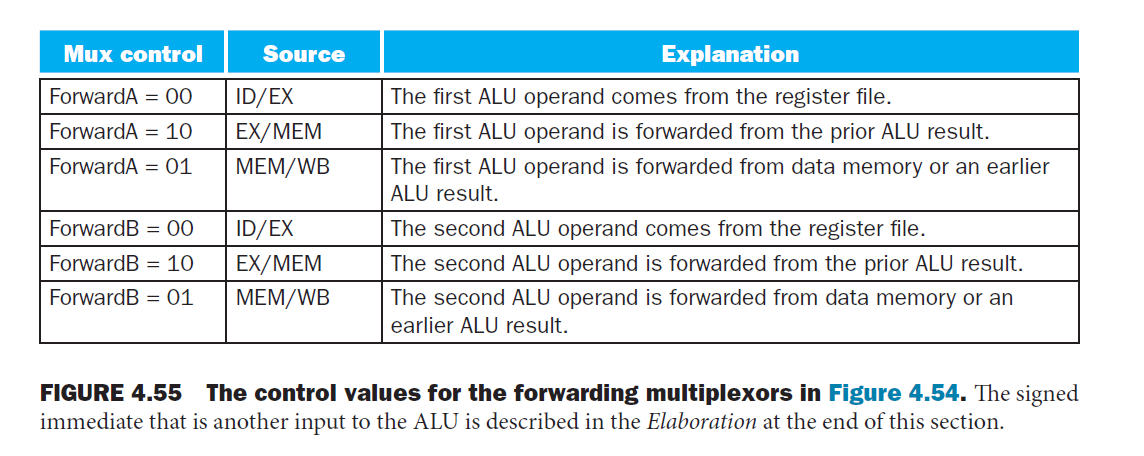
\includegraphics[scale=0.5]{Images/forwarding_mux_values.png}
\caption{Forwarding (mux values)}
\end{figure}

\begin{figure}[h]
\centering
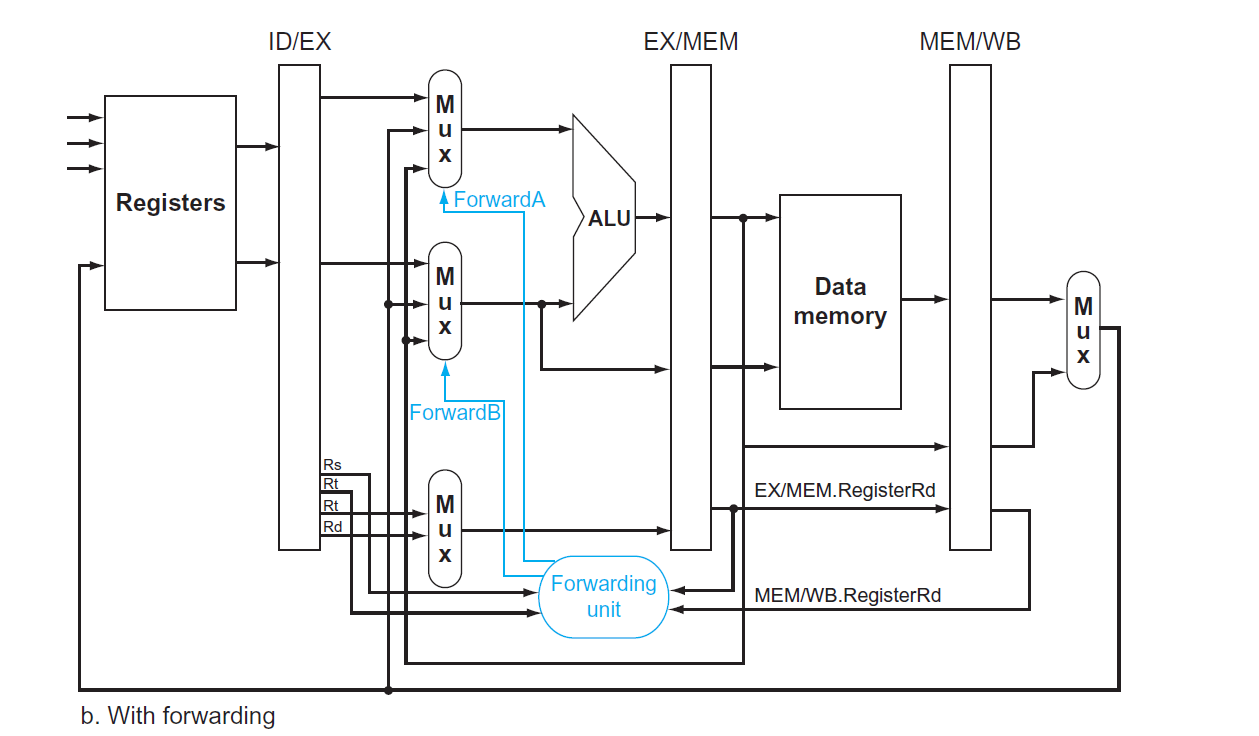
\includegraphics[scale=0.5]{Images/forwarding.png}
\caption{Forwarding unit for a pipeline}
\end{figure}

\begin{figure}[h]
\centering
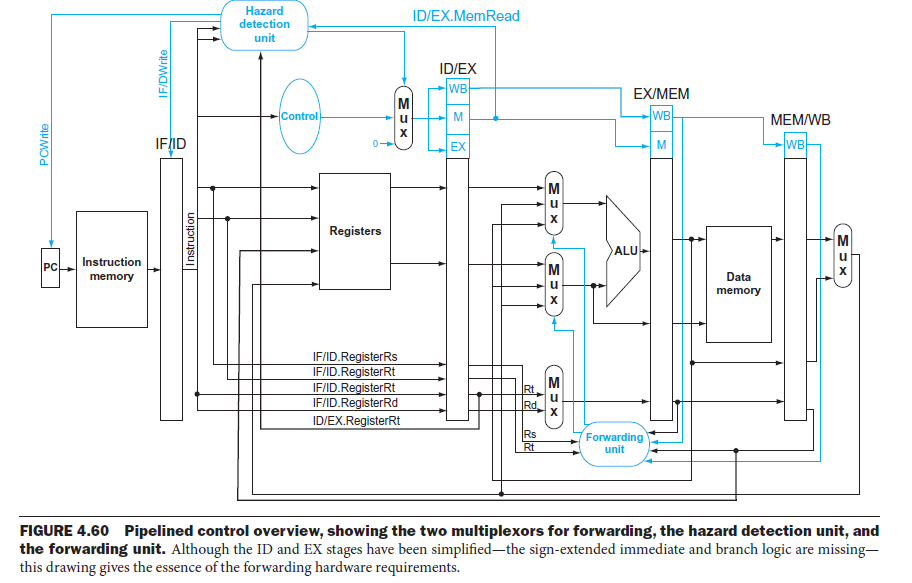
\includegraphics[scale=0.6]{Images/hazard+fwding.png}
\caption{Hazard and forwarding unit for a pipeline}
\end{figure}

\begin{figure}[h]
\centering
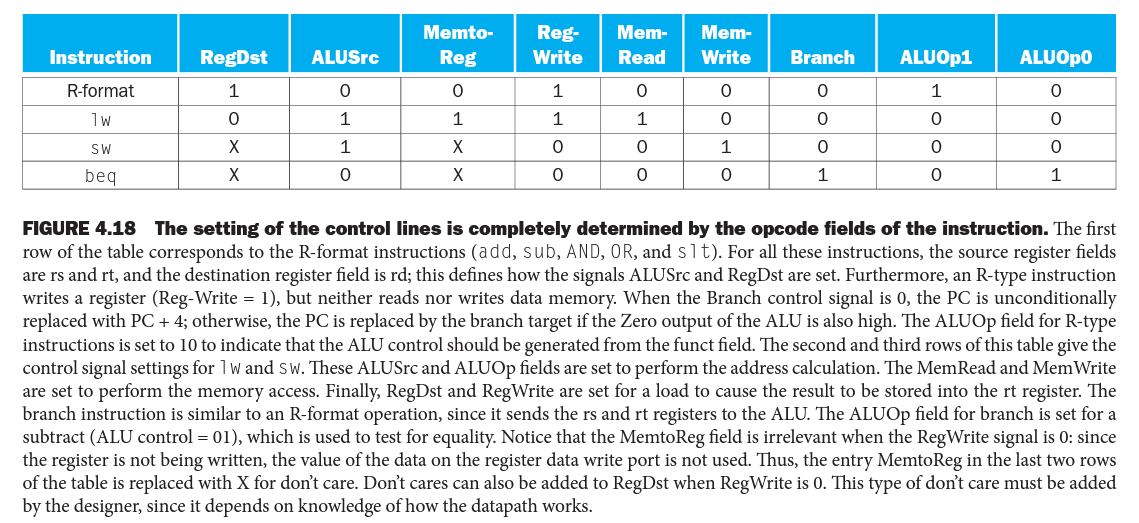
\includegraphics[scale=0.5]{Images/inst_to_signals.png}
\caption{Instruction type to control signals in a MIPS instruction set}
\end{figure}

\begin{figure}[h]
\centering
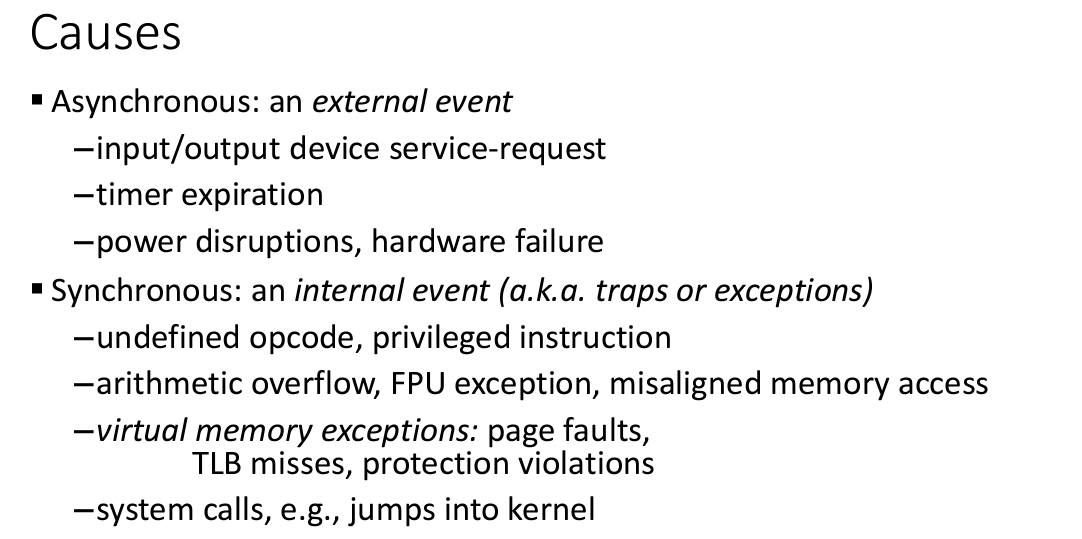
\includegraphics[scale=0.5]{Images/interrupt_causes.png}
\caption{Causes of interrups}
\end{figure}

\begin{figure}[h]
\centering
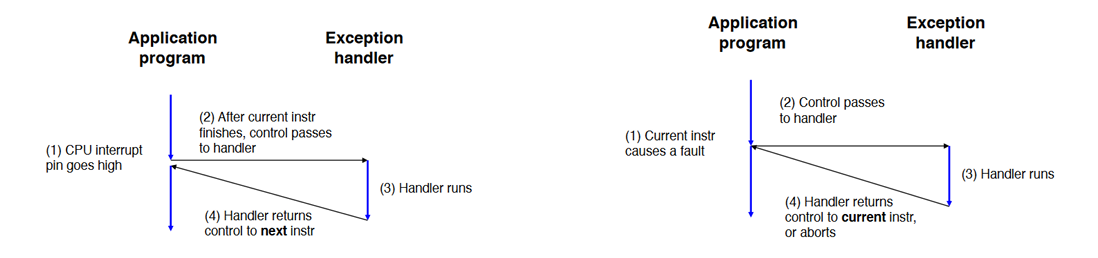
\includegraphics[scale=0.5]{Images/interrupt_exec.png}
\caption{Interrupt handling for a program}
\end{figure}

\begin{figure}[h]
\centering
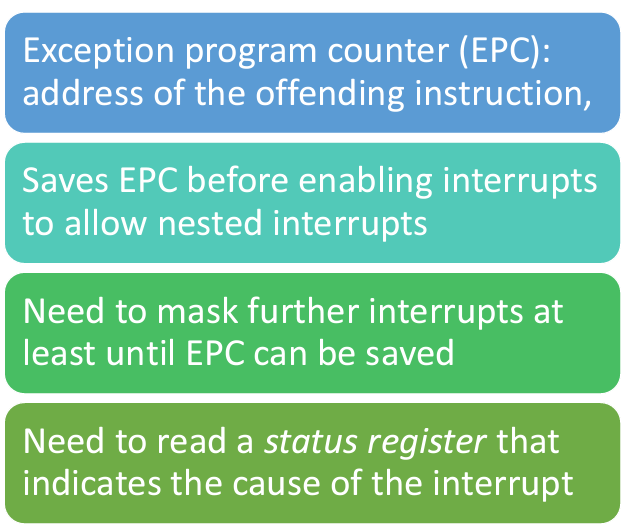
\includegraphics[scale=0.5]{Images/interrupt_handler_1.png}
\caption{Exception program counter (interrupt handler)}
\end{figure}

\begin{figure}[h]
\centering
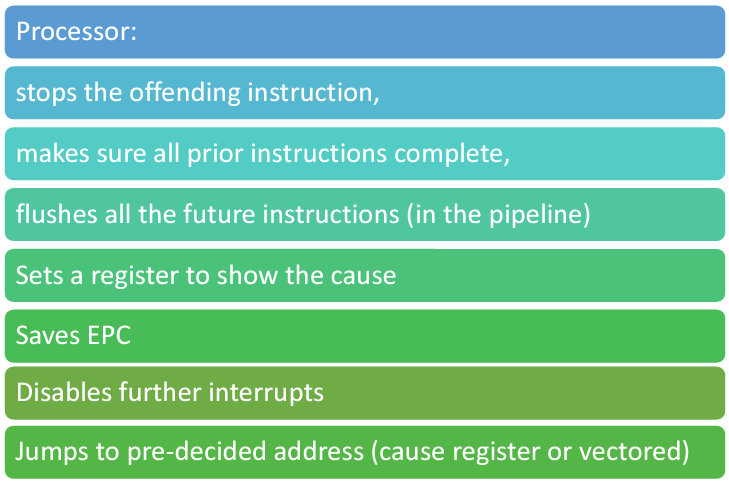
\includegraphics[scale=0.5]{Images/interrupt_handler_2.png}
\caption{Processor's role (interrupt handler)}
\end{figure}

\begin{figure}[h]
\centering
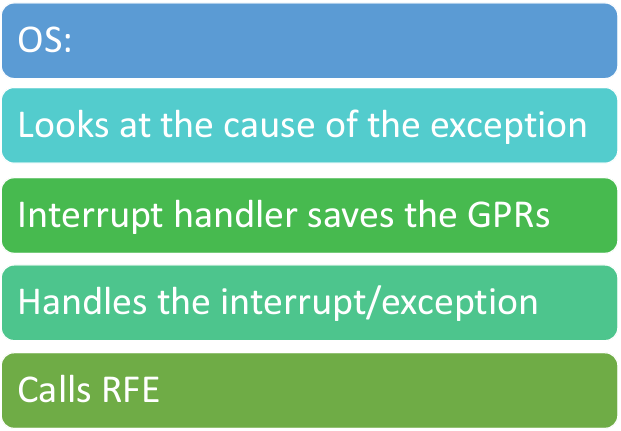
\includegraphics[scale=0.5]{Images/interrupt_handler_3.png}
\caption{OS's role (interrupt handler)}
\end{figure}

\begin{figure}[h]
\centering
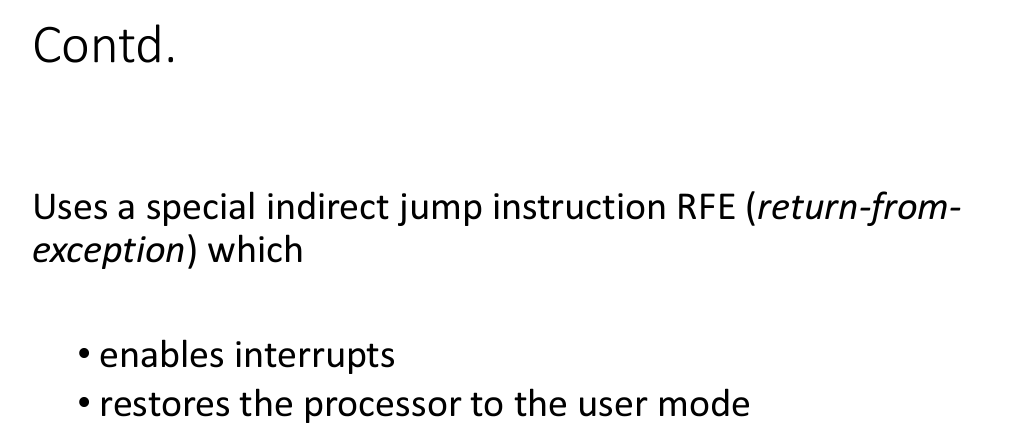
\includegraphics[scale=0.5]{Images/interrupt_handler_4.png}
\caption{RFE instruction for exception handling (interrupt handler)}
\end{figure}

\begin{figure}[h]
\centering
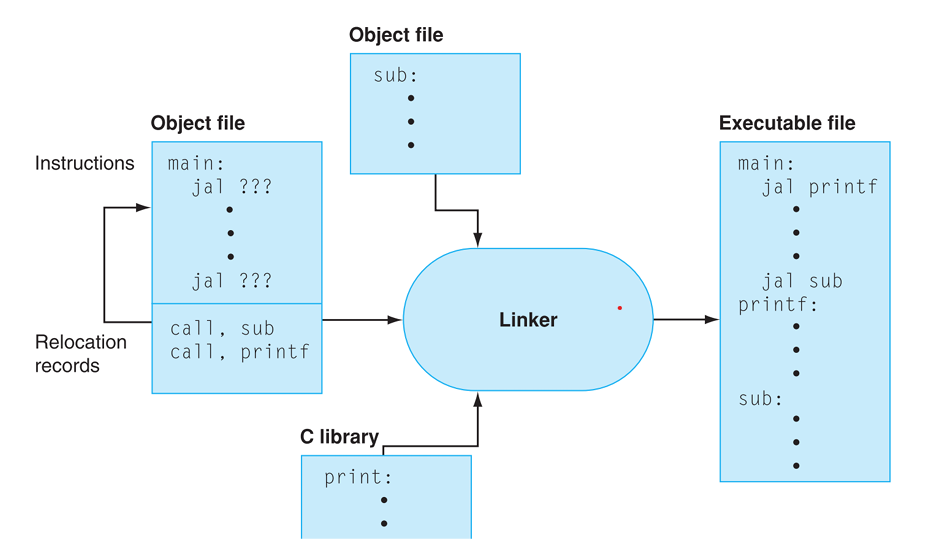
\includegraphics[scale=0.5]{Images/linker.png}
\caption{Linker (diagrammatic depiction)}
\end{figure}

\begin{figure}[h]
\centering
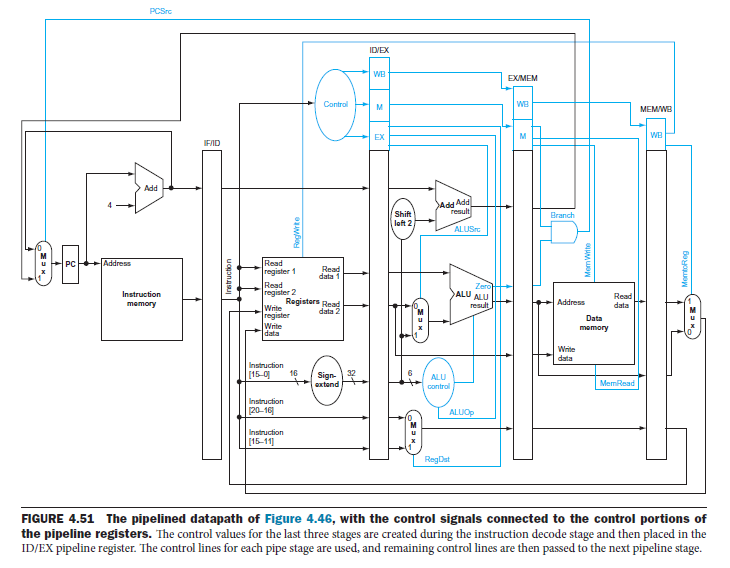
\includegraphics[scale=0.6]{Images/pipeline.png}
\caption{A pipeline with all control signals}
\end{figure}

\begin{figure}[h]
\centering
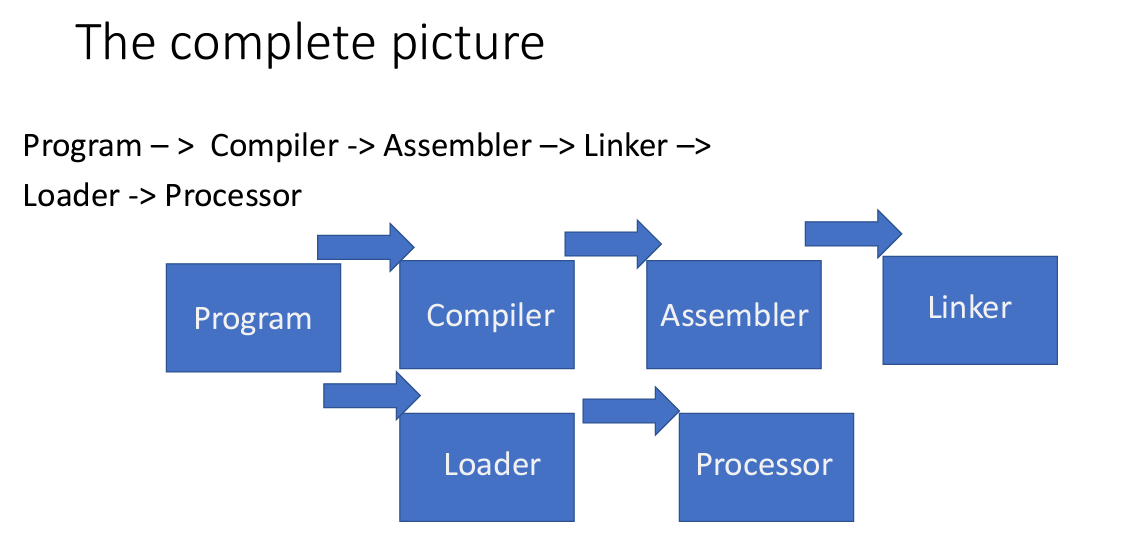
\includegraphics[scale=0.5]{Images/program_processor.png}
\caption{The complete path of ``agents (programs/components)" from a program to an executable}
\end{figure}

\begin{figure}[h]
\centering
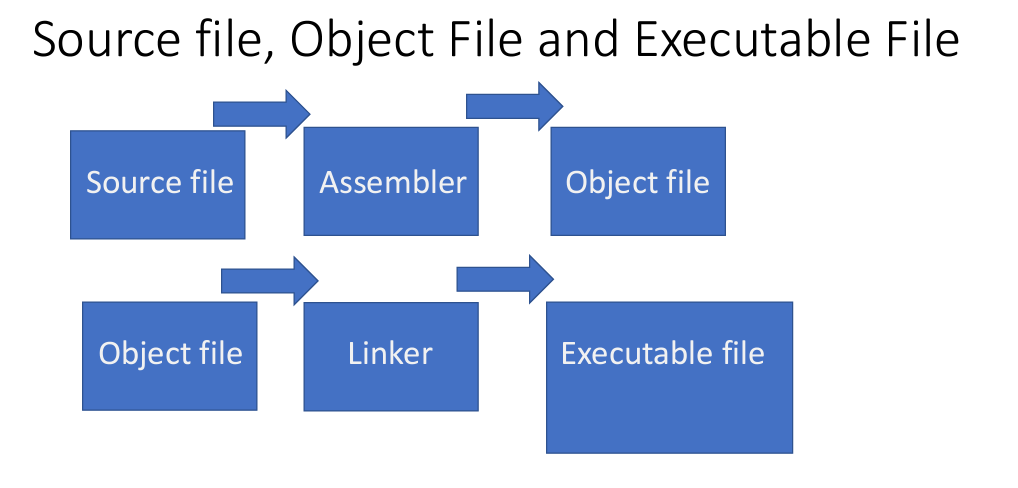
\includegraphics[scale=0.5]{Images/source_exec.png}
\caption{The path of files from source file to executable}
\end{figure}

\end{document}

